%!TEX root = ../template.tex
%%%%%%%%%%%%%%%%%%%%%%%%%%%%%%%%%%%%%%%%%%%%%%%%%%%%%%%%%%%%%%%%%%%%
%% chapter3.tex
%% NOVA thesis document file
%%
%% Chapter with a short latex tutorial and examples
%%%%%%%%%%%%%%%%%%%%%%%%%%%%%%%%%%%%%%%%%%%%%%%%%%%%%%%%%%%%%%%%%%%%

\typeout{NT FILE chapter3.tex}%


\chapter{Materials and Methods}
\label{cha:materials_and_methods}

\section{Gene expression data} % (fold)
\label{sec:gene_expression_data}


%\includegraphics[width=0.9\linewidth]{Chapters/Figures/lincs_shrna_a375_head(signature)}\hfill


\begin{figure}[htbp]
    \centering
    \includegraphics[height=2in]{lincs_shrna_a375_head(signature)}
    \caption{Transctipotomic signatures perturbation from LINCS shRNA, cell line a375.}
    \label{fig:example_signatures}
\end{figure}


The Table ~\ref{tab:dataset_summary} provides a summary od the datasets used in the study.

\bgroup
%\rowcolors{1}{}{GhostWhite}
\begin{xltabular}{\textwidth}{Xccccc}
    \caption{Datasets summary.}
    \label{tab:dataset_summary}\\
    \toprule
    %\rowcolor{Gainsboro}%
    \textbf{Dataset}                & \textbf{Perturbagen}     & \textbf{Perturbation}  & \textbf{N. of perturbagens}    & \textbf{Signature} \\
    \midrule
LINCS compounds            & Chemical        & Compound      & 3499                  & Full      \\
LINCS CRISPR               & Genetic         & CRISPR KO     & \emph{2B, 1C}         & Full      \\
LINCS OE                   & Genetic         & ?             & \emph{A}              & Full      \\
LINCS shRNA a375           & Genetic         & ?             & ---                   & Full      \\
ChemPert                   & Chemical        & 2             & \emph{C}              & DEGs      \\
CREEDs                     & Chemical        & 2             & \emph{1A, 1C}         & 0 \\
CDS-DB                     & Chemical        & 1             & ---                   & 0 \\
PertOrg                    & Genetic         & 1             & \emph{1A}             & 0 \\
GWPS                       & Genetic         & 2             & \emph{C}              & 0 \\
Sci-Plex                   & Chemical        & 3             & \emph{2B}             & 0 \\
%\midrule
%\rowcolor{Gainsboro}%
    \bottomrule
    \end{xltabular}
\egroup


\section{Biological Network} % (fold)
\label{sec:biological_network}



\section{Algortithms} % (fold)
\label{sec:algorithms}

The Table ~\ref{tab:algorithm_summary} provides a summary od the algorithms used in the study.

%% If I need to change this table to a horizontal layout, just uncomment the next line and the line after the table:
%% \begin{newpdflayout}{210mm}{297mm}%{420mm}

\bgroup
%\rowcolors{1}{}{GhostWhite}
\begin{xltabular}{\textwidth}{Xccccc}
\caption{Algorithm summary.}
\label{tab:algorithm_summary}\\
\toprule
%\rowcolor{Gainsboro}%
\textbf{Tool}  & \textbf{Algorithm}   & \textbf{Description}   & \textbf{Resource}   & \textbf{Dataset}   & \textbf{Reference}   \\
\midrul
\multicolumn{8}{*}{\multirow{2}{*}{\textbf{Causal Reasoning}}}    & CARNIVAL            & Description  & Network    & DEG/Full  & ~\cite{carnival} \\
                & CausalR             & Description  &            &           & ~\cite{causalr} \\
                & ProTINA             & Description  &            &           & ~\cite{protina} \\
                & CIE                 & Description  &            &           & ~\cite{cie} \\
                & NicheNet            & Description  &            &           & ~\cite{nichenet} \\
                & causalReasoning     & Description  &            &           & ~\cite{cbdd} \\
                & Signatures          & Description  &            &           & ~\cite{cbdd} \\
                & quaternaryProd      & Description  &            &           & ~\cite{cbdd} \\    
\midrule
\textbf{Causal}     & randomWalk          & Description  & Network    & DEG/Full  & ~\cite{cbdd} \\
\textbf{Reasoning}  & networkPropagation  & Description  &            &           & ~\cite{cbdd} \\
(baseline)          & overconnectivity    & Description  &            &           & ~\cite{cbdd} \\
                & hiddenNodes         & Description  &            &           & ~\cite{cbdd} \\
                & interconnectivity   & Description  &            &           & ~\cite{cbdd} \\
                & overconnectivity    & Description  &            &           & ~\cite{cbdd} \\
\midrule
\textbf{CMap}       & KS             & Description & Signatures   & DEG/Full     & ~\cite{cmap} \\
                & XCos           & Description &              &              & ~\cite{cmap} \\
                & XSum           & Description &              &              & ~\cite{cmap} \\
                & ZhangScore     & Description &              &              & ~\cite{cmap} \\
                & GSEAweight0    & Description &              &              & ~\cite{cmap} \\
                & GSEAweight1    & Description &              &              & ~\cite{cmap} \\
\midrule
\textbf{Enrichment} & wmean   & Description  & Regulons     & Signatures  & ~\cite{cbdd} \\
                & fgsea   & Description  &              &             & ~\cite{fgsea} \\
                & viper   & Description  &              &             & ~\cite{viper} \\
                & ulm     & Description  &              &             & ~\cite{cbdd} \\
                & mlm     & Description  &              &             & ~\cite{cbdd} \\
                & udt     & Description  &              &             & ~\cite{cbdd} \\
                & mdt     & Description  &              &             & ~\cite{cbdd} \\
                & wsum    & Description  &              &             & ~\cite{fgsea} \\
%\rowcolor{Gainsboro}%
\bottomrule
\end{xltabular}
\egroup


%\end{newpdflayout}
